

\documentclass{beamer}
\usetheme{Madrid}
\usepackage{xeCJK}  % 中文支持
\setCJKmainfont{SimHei}
\usecolortheme{seahorse}
\usepackage{amsmath,amssymb}
\usepackage{graphicx}
\usepackage{tikz}
\usepackage{hyperref}
\usepackage{booktabs}
\usepackage{multirow}
\usepackage{multicol}
\usepackage{xcolor}
\usepackage{subcaption}
\usepackage{float}
\usepackage{listings}
\usepackage{longtable}
\usepackage{booktabs}
\usepackage{threeparttable}
\usepackage{array}
\usepackage{makecell}
\usepackage{siunitx}
\usepackage{gensymb}
\usepackage{pgfplots}
\usepackage{pgfplotstable}
\usepackage{pgfplotstable}
\usepackage{pgfplotstable}
\usepackage{pgfplots}
\usepackage{pgfplotstable}
\usepackage{pgfplotstable}
\usepackage{pgfplotstable}
\usepackage{pgfplots}
\usepackage{pgfplotstable}
\usepackage{pgfplotstable}
\usepackage{pgfplots}
\usepackage{pgfplotstable}
\usepackage{pgfplotstable}
\usepackage{pgfplots}
\usepackage{pgfplotstable}
\usepackage{pgfplotstable}
\usepackage{pgfplots}
\usepackage{pgfplotstable}
\title{全球通胀溢出的多频率网络与动态社区演化}
\subtitle{基于GAT图嵌入的谱聚类测度}
\author{林晟}
\institute{统计学院}
\date{\today}

\begin{document}

\frame{\titlepage}

\begin{frame}{以往研究及背景}
  \begin{block}{现实问题}
    在全球化背景下,通胀的跨国溢出机制分析与国际驱动因素识别已逐步成为宏观经济的热点问题。系列重大突发事件导致跨国供应链停滞、能源价格上涨以及多国颁布\textbf{扩张性财政货币政策},进而导致全球通货膨胀水平飙升,经济滞胀的风险大幅提升。
  \end{block}

  \begin{itemize}
    \item 主要聚焦通货膨胀的整体风险或个别极端事件(如COVID-19、俄乌冲突)。
    \item 研究特定历史时期中极端事件冲击带来的通货膨胀及其溢出效应。
    \item 聚焦代表性国家如G7、G20,研究范围相对较小,往往忽视经济体量小但在金融、原材料、进出口领域发挥重要作用的国家。
    \item 大多数研究基于短期影响(月度数据)。
    \item 经济体分类依赖于先验知识,如按国际组织或行业划分,缺乏数据驱动的方法。
  \end{itemize}
\end{frame}


\begin{frame}{创新点与待解决问题}
  \begin{block}{待解决问题}
    \begin{itemize}
      \item 如何解决高维估计问题以更有效地识别并更多经济体在全球通胀中的作用?
      \item 如何从混频的角度全面理解国际通货膨胀的溢出效应?
      \item 如何实现对社区内外通胀不平等的精确测度和影响分析?
    \end{itemize}
    \vspace{0.2cm}
  \begin{block}{创新点}
    \begin{itemize}
      \item 扩大研究对象,包括在全球通货膨胀中起重要作用的小型经济体。
      \item 引入长期因素进行讨论,考虑网络溢出的混频影响。
      \item 测度并研究国际通货膨胀中的社区性不平等现象。
      \item 应用图神经网络(GAT)提供更有效的参数估计方式,以估计高维的长短期溢出网络。
    \end{itemize}
  \end{block}


  \end{block}
\end{frame}


\begin{frame}{典型事实}
  \centering
  \begin{columns}
    \column{0.5\textwidth}
    \centering
    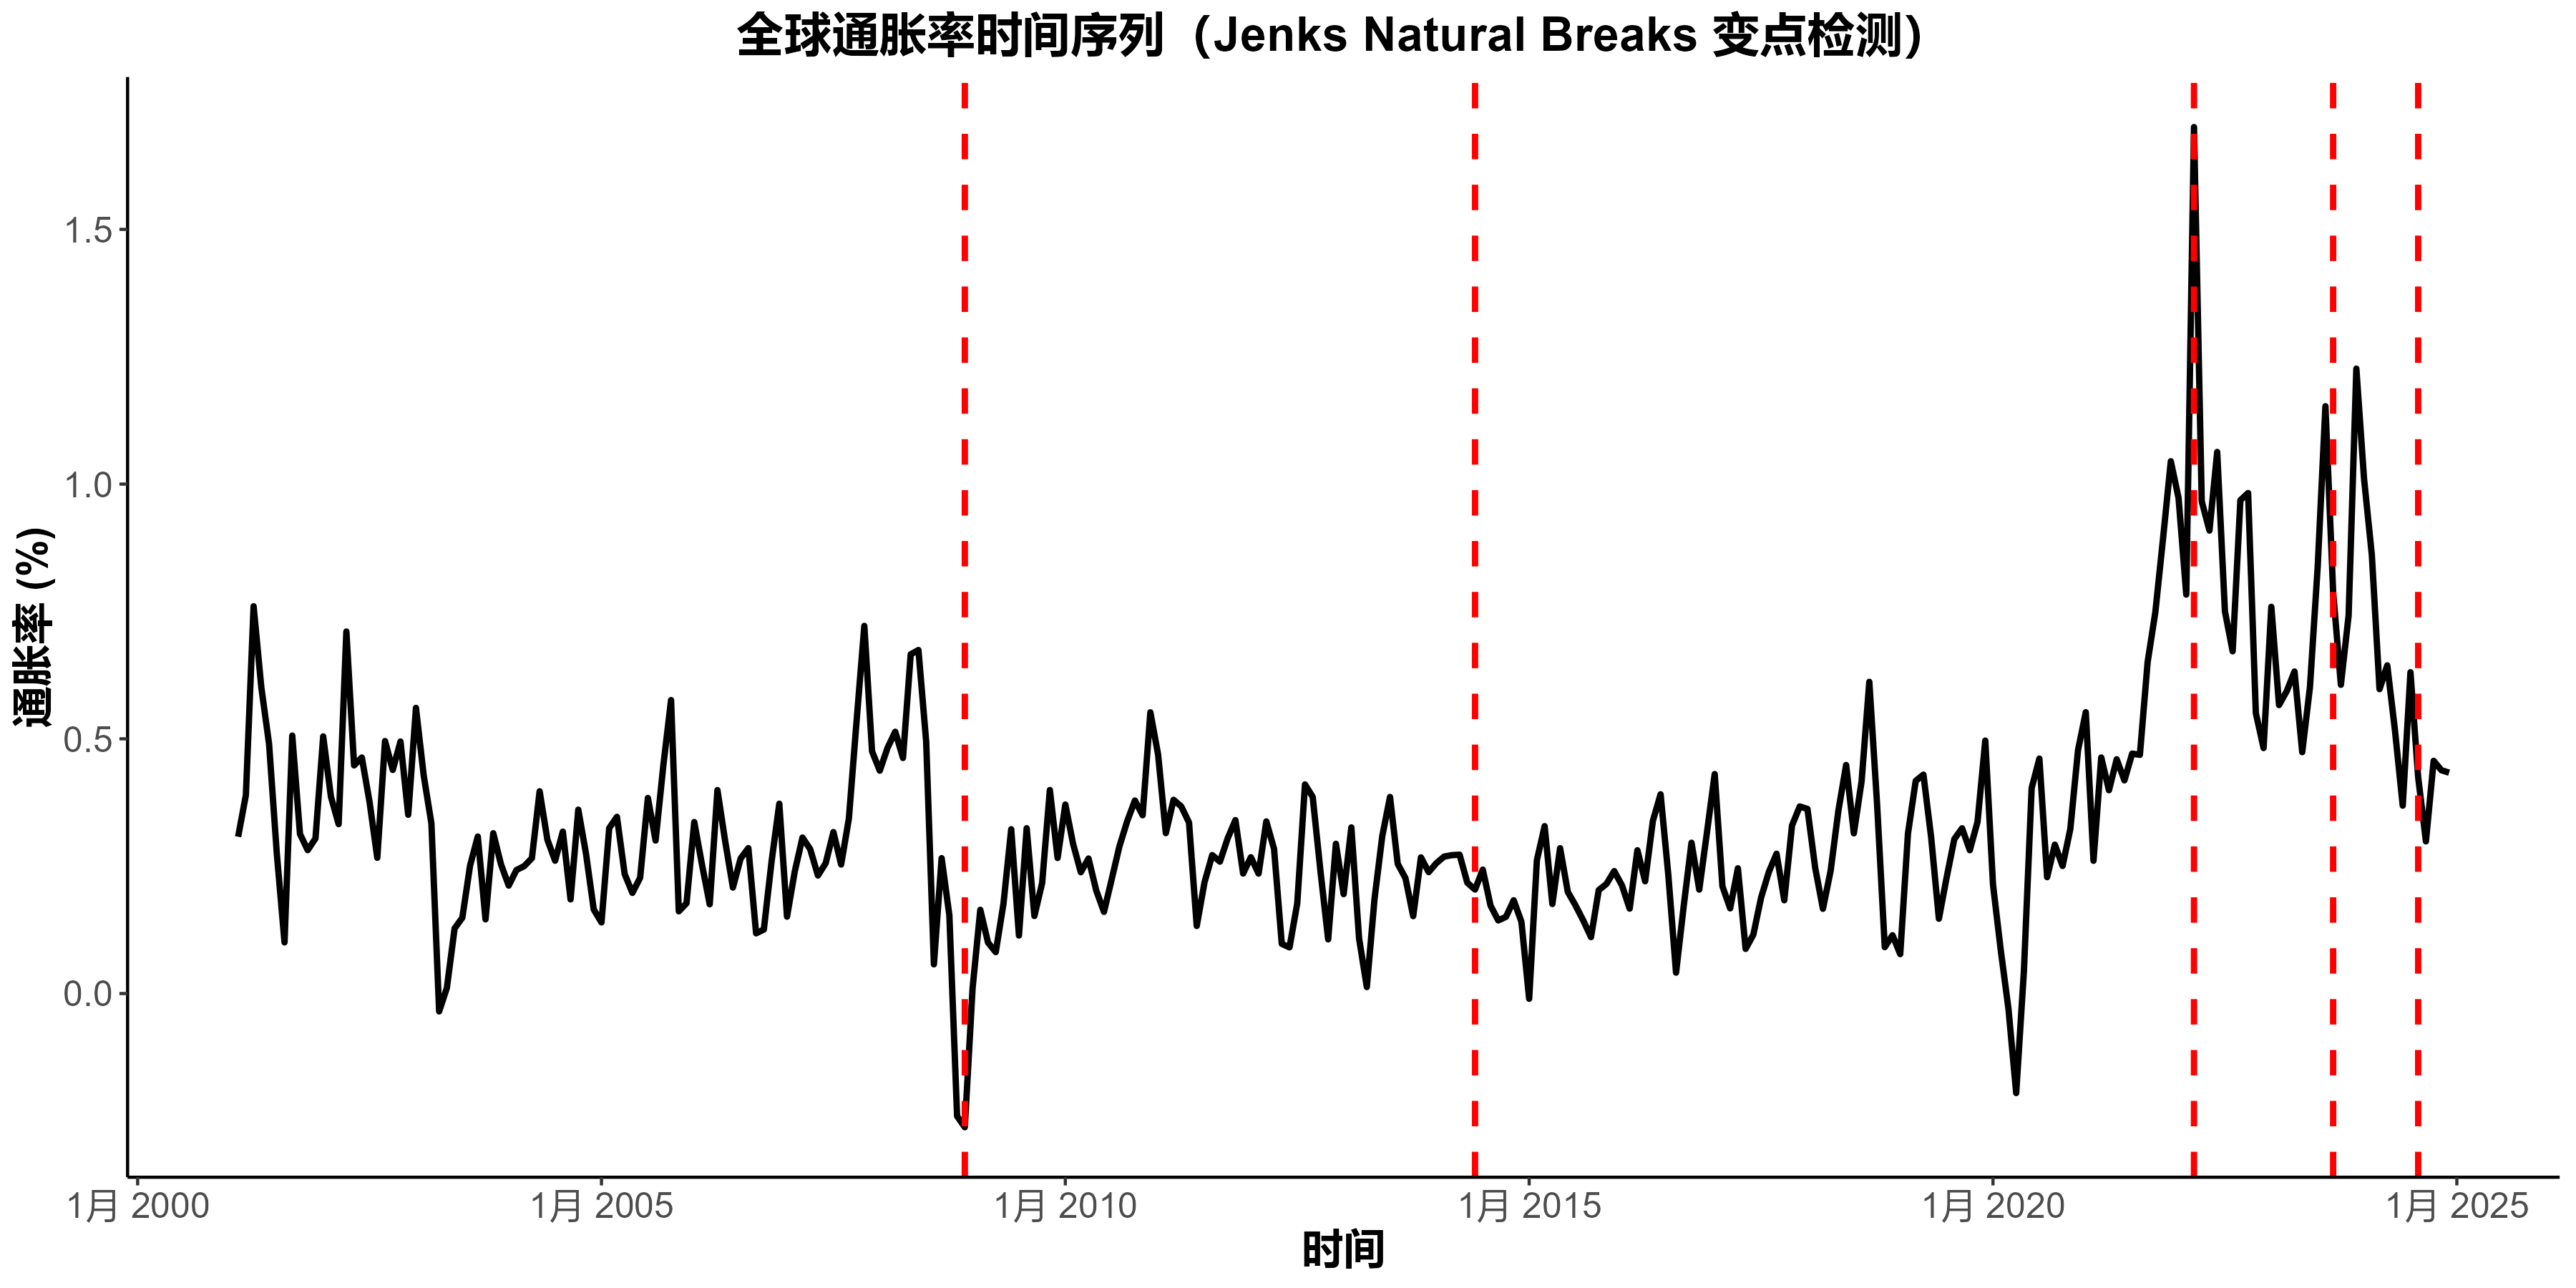
\includegraphics[width=\linewidth]{fig/Inflation_Jenks.png}
    \textbf{(a) 全球通胀率平均趋势}
    
    \column{0.5\textwidth}
    \centering
    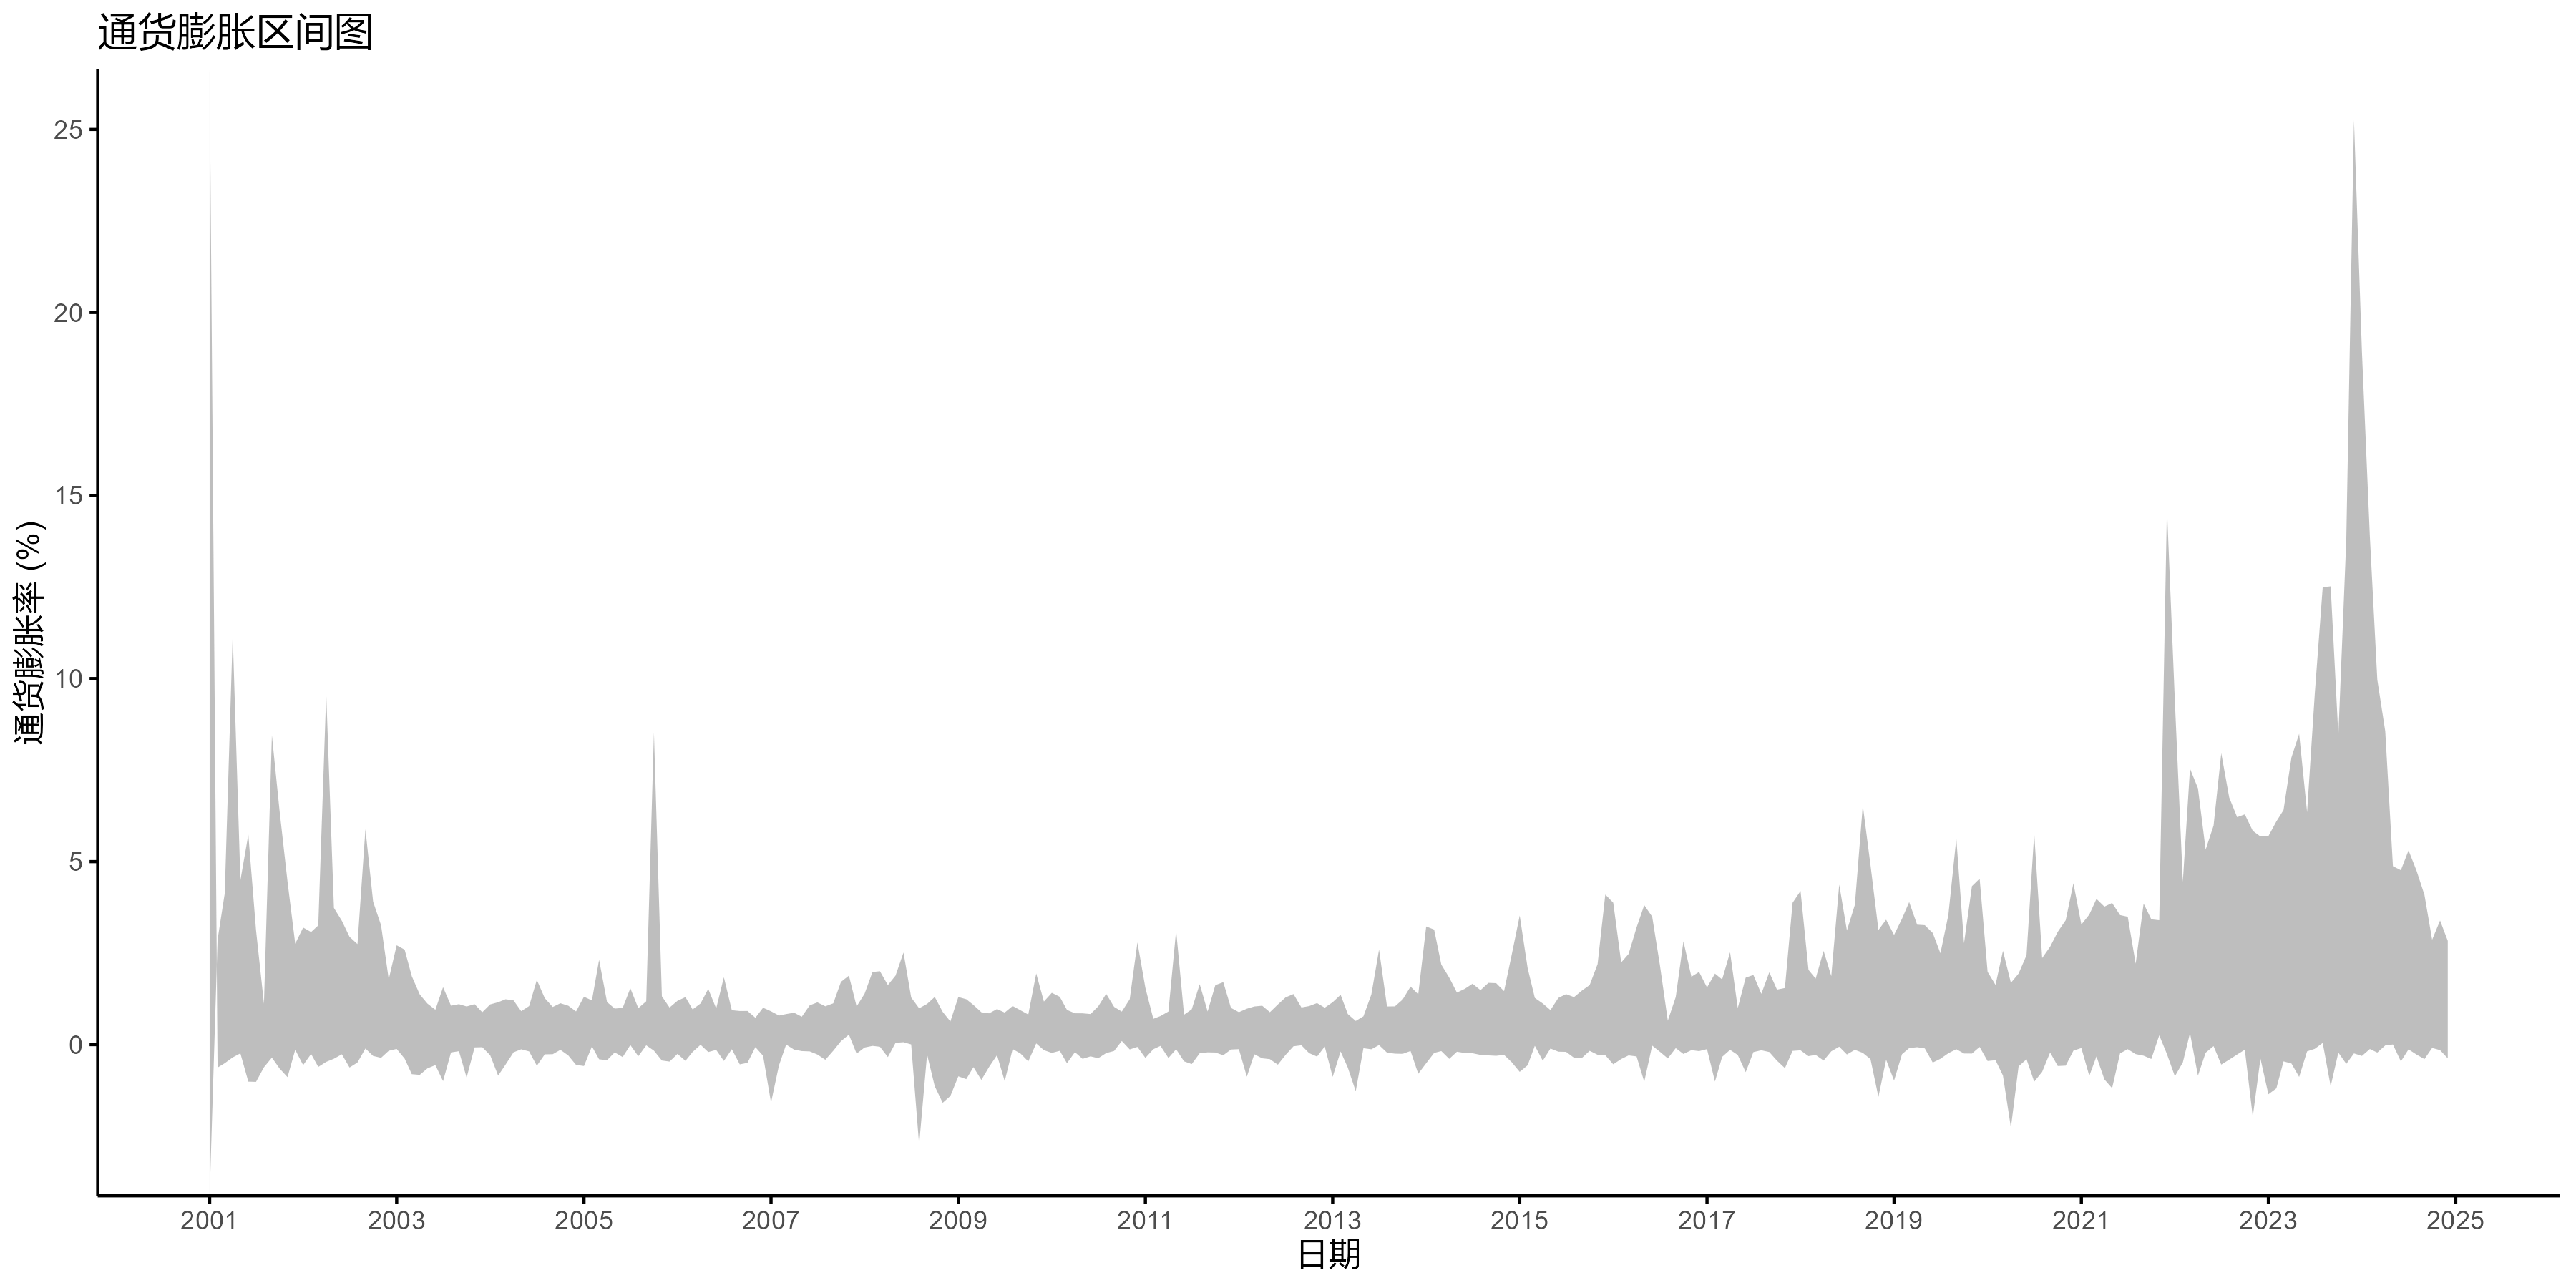
\includegraphics[width=\linewidth]{fig/Inflation_TimeSeries.png}
    \textbf{(b) 全球通胀率区间}
  \end{columns}

  \vspace{0.5cm} % 添加一些垂直空间
  \begin{block}{核心发现}
  \begin{itemize}
    \item 全球通胀水平显著提高
    \item 全球通胀风险近年来明显加剧
  \end{itemize}
\end{block}
\end{frame}



\begin{frame}{典型事实}
  \centering
  \begin{columns}
    \column{0.5\textwidth}
    \centering
    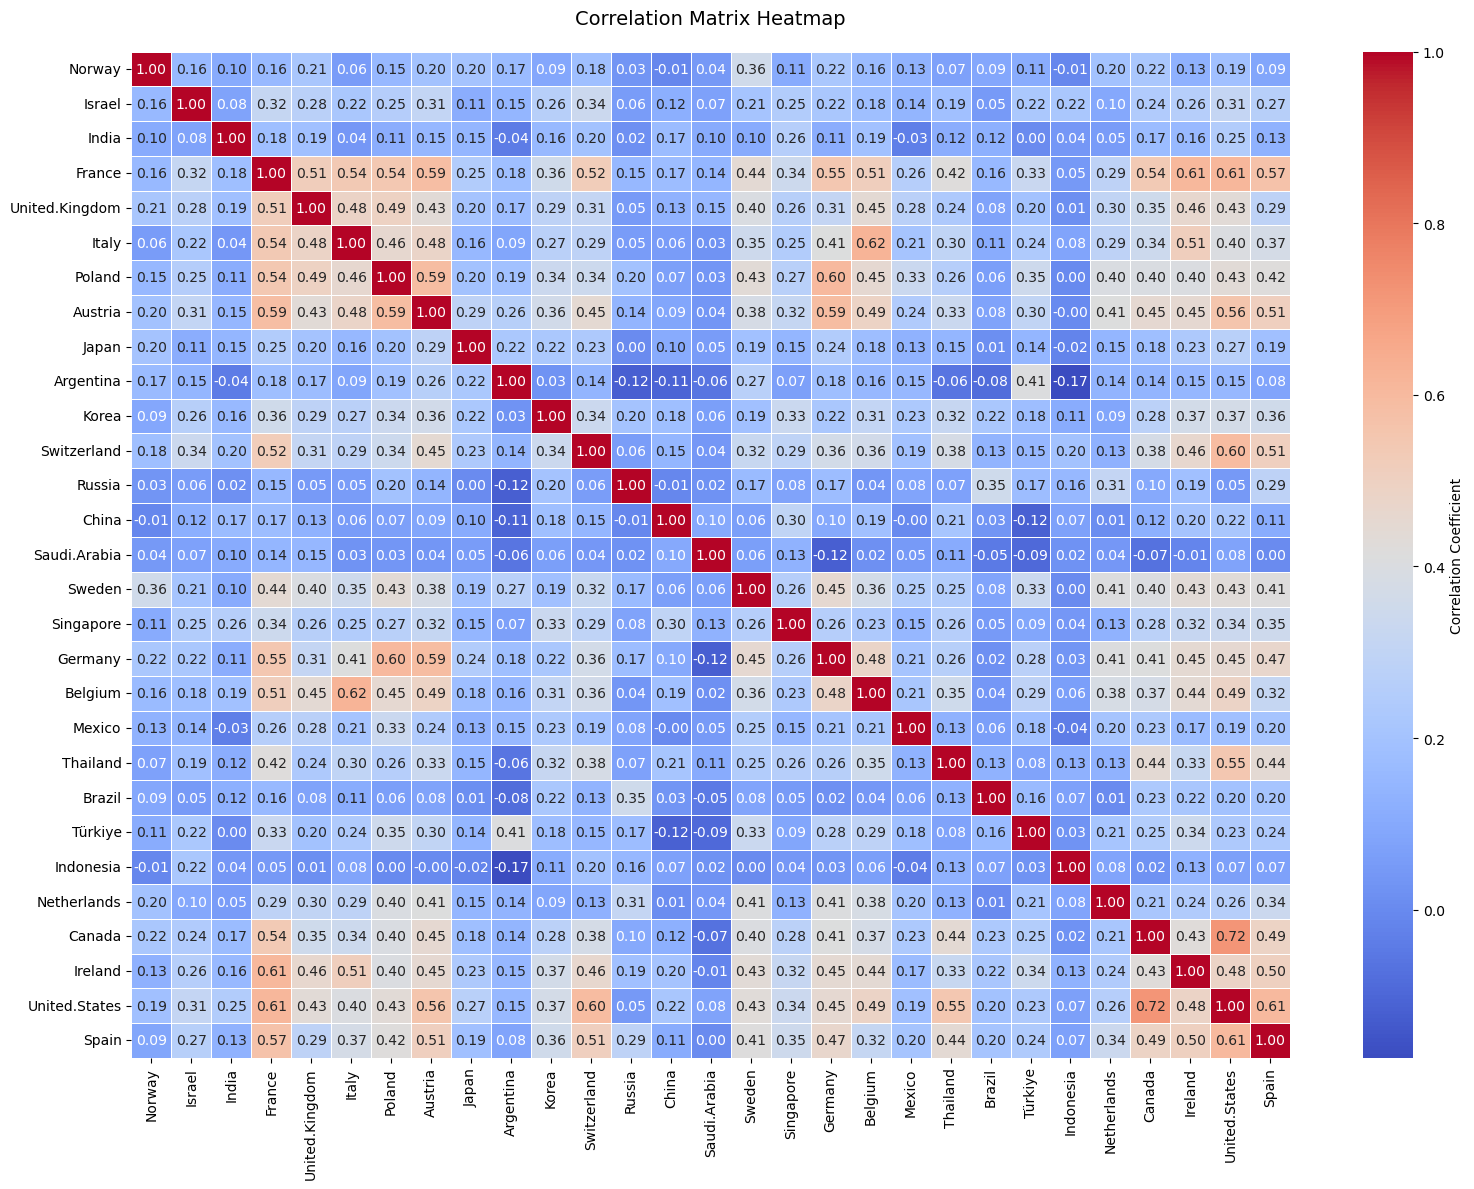
\includegraphics[width=\linewidth]{fig/Inflation_CorrelationHeatmap.png}
    \textbf{(a) 全球通胀相关性热力图}
    
    \column{0.5\textwidth}
    \centering
    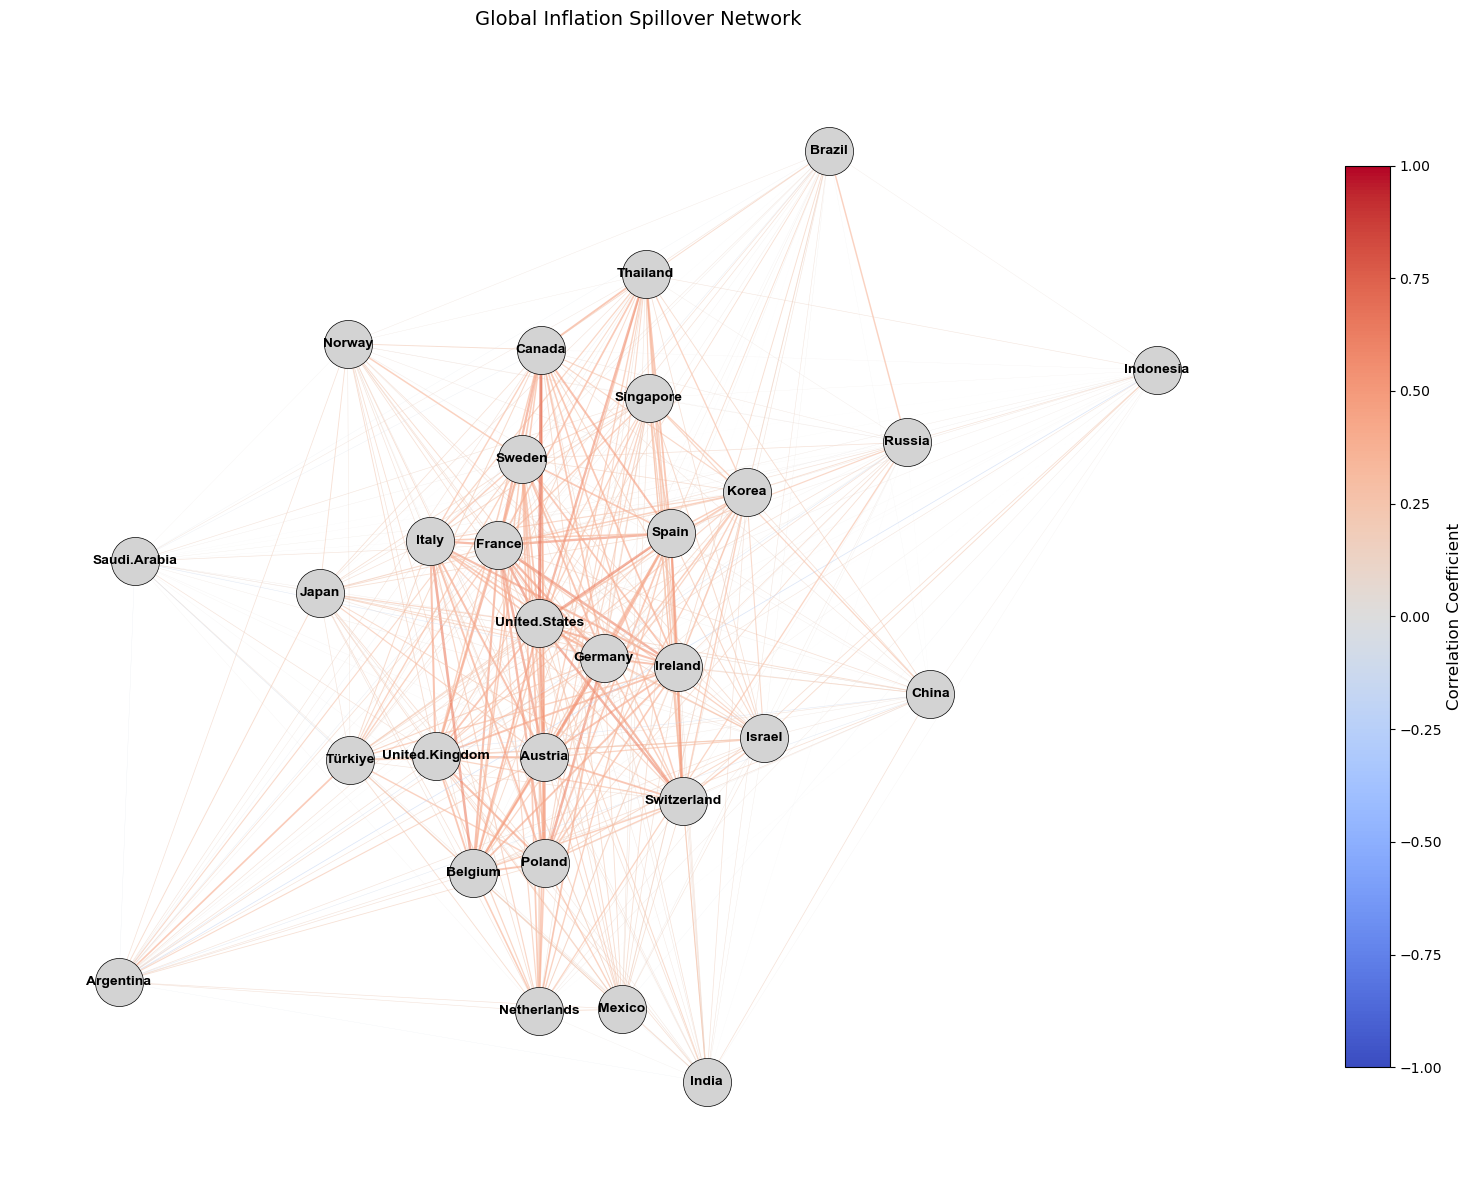
\includegraphics[width=\linewidth]{fig/Inflation_NetworkGraph.png}
    \textbf{(b) 全球通胀网络图}
  \end{columns}

  \vspace{0.1cm} % 添加一些垂直空间

  \begin{block}{核心发现}
    \begin{itemize}
      \item 全球通胀连接相关性紧密,显示出高度的互动性。
      \item 呈现核心-边缘社区特征,部分经济体在全球通胀动态中起核心作用。
    \end{itemize}
  \end{block}
\end{frame}

\begin{frame}{研究意义}
  \begin{itemize}
    \item \textbf{理论贡献}:通过引入新的数据驱动方法和长期分析视角,本研究为理解通货膨胀的跨国溢出效应提供了新的理论框架。特别是在包括小型经济体和考虑非传统因素的情境下,扩展了传统宏观经济模型。
    
    \item \textbf{政策影响}:研究结果可以为政策制定者提供更精确的工具,以预测和应对国际通货膨胀的影响。尤其是在全球经济危机情况下,能够更好地制定包容性财政和货币政策。
    
    \item \textbf{经济预测}:通过改进通货膨胀预测模型,本研究提高了经济预测的准确性,特别是在全球或区域经济不稳定期间。这有助于经济决策者和市场参与者更好地制定策略。
    
    \item \textbf{社会贡献}:提高对经济波动敏感的小型国家的可见度,有助于全球经济治理中更公平的声音分配。这可能导致更平衡的全球经济政策,从而促进全球经济的稳定性和包容性。
  \end{itemize}
\end{frame}
% 核心模型:TVP-VHAR
\begin{frame}{核心模型:TVP-VHAR}
\textbf{传统VHAR模型} (Corsi 2009):
\begin{equation*}
\boldsymbol{y}_t = \beta_0 + \beta_d \boldsymbol{y}_{t-1} + \beta_w \frac{1}{5}\sum_{i=1}^5 \boldsymbol{y}_{t-i} + \beta_m \frac{1}{22}\sum_{i=1}^{22} \boldsymbol{y}_{t-i} + \epsilon_t
\end{equation*}

\textbf{时变扩展 (TVP-VHAR)}:
\begin{gather*}
\boldsymbol{y}_t = \beta_{0,t}  + \beta_{m,t} \boldsymbol{y}_{t}^{(m)} + \beta_{y,t} \boldsymbol{y}_{t}^{(y)} + \epsilon_t \\
\boldsymbol{\beta}_t = \boldsymbol{\beta}_{t-1} + \boldsymbol{\nu}_t, \quad \boldsymbol{\nu}_t \sim N(0,\boldsymbol{Q})
\end{gather*}
其中:
\begin{itemize}
\item $\boldsymbol{y}_{t}^{(m)} = \sum_{i=1}^5 \boldsymbol{y}_{t-i}$(月度成分)
\item $\boldsymbol{y}_{t}^{(y)} = \sum_{i=1}^{22} \boldsymbol{y}_{t-i}$(年度成分)
\end{itemize}
\end{frame}



% 动态网络构建
\begin{frame}{动态网络构建}
\textbf{邻接矩阵} (时变溢出强度):
\begin{equation*}
A_t = (O_t)^{-\frac{1}{2}}\Phi_t(P_t)^{-\frac{1}{2}}
\end{equation*}

\textbf{标准化Laplacian矩阵}:
\begin{equation*}
\mathcal{L}_t = \boldsymbol{D}_t^{-1/2} (\boldsymbol{D}_t - \boldsymbol{A}_t) \boldsymbol{D}_t^{-1/2}
\end{equation*}
其中$\boldsymbol{D}_t = \text{diag}(\sum_j A_t(i,j))$为度矩阵
\end{frame}

% 社区检测
\begin{frame}{社区检测:谱聚类+k-means}
\textbf{SVD分解}:
\begin{equation*}
\mathcal{L}_t = \boldsymbol{U}_t \boldsymbol{\Sigma}_t \boldsymbol{V}_t^\top
\end{equation*}
取前$k$个左/右奇异向量 $\boldsymbol{U}_t^{(k)}, \boldsymbol{V}_t^{(k)}$

\textbf{双向聚类}:
\begin{align*}
\text{发送社区: } & \text{k-means}(\boldsymbol{U}_t^{(k)}) \\
\text{接收社区: } & \text{k-means}(\boldsymbol{V}_t^{(k)})
\end{align*}
\end{frame}

\begin{frame}{可行性及进展}
  \begin{block}{研究方法的可行性}
    \begin{itemize}
      \item 利用神经网络的计算能力,有效追踪和分析短期和长期通货膨胀的全球溢出效应。
      \item 数据采用国际清算银行核算结果,保证有效性和可得性
    \end{itemize}
  \end{block}

  \begin{figure}
    \centering
    \begin{minipage}{0.48\textwidth}
      \centering
      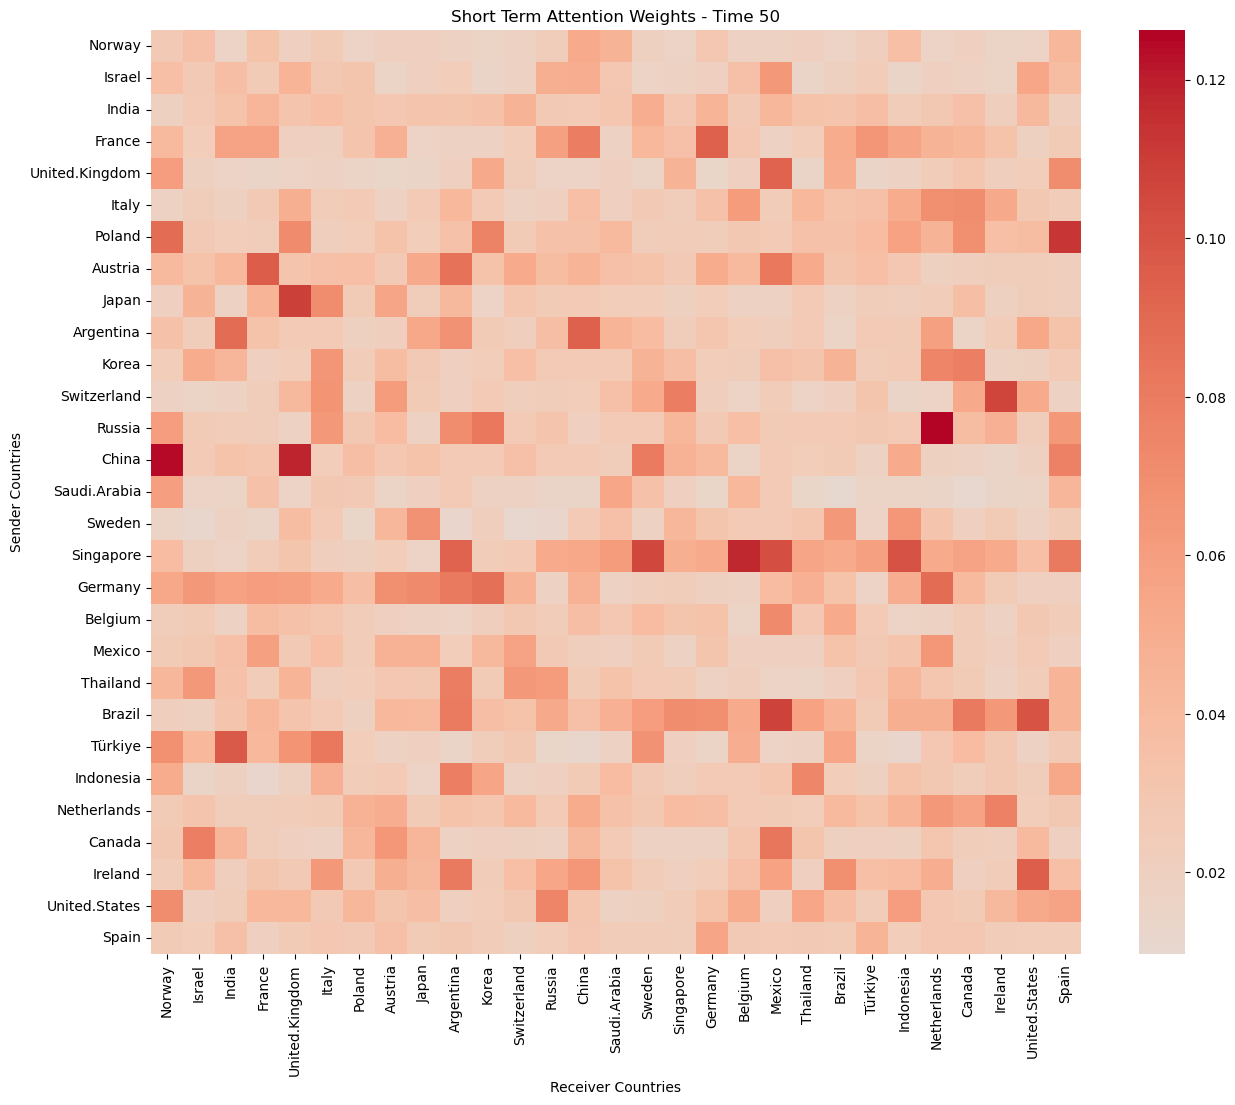
\includegraphics[width=\textwidth]{fig/short_term_spillover_heatmap.png}
      \caption{短期通货膨胀溢出热力图}
    \end{minipage}
    \hfill
    \begin{minipage}{0.48\textwidth}
      \centering
      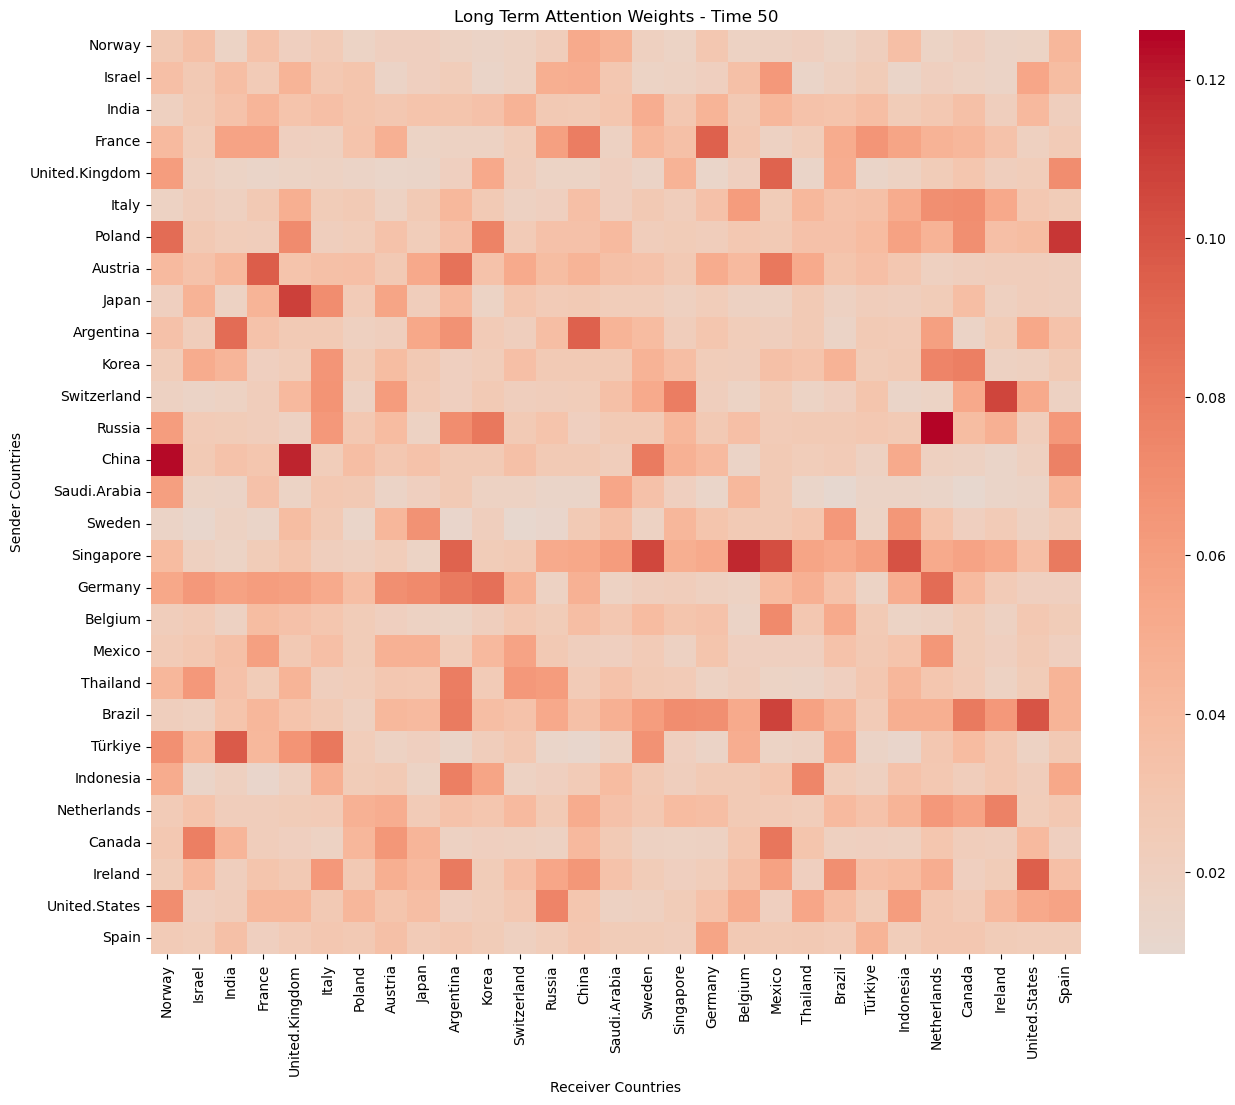
\includegraphics[width=\textwidth]{fig/long_term_spillover_heatmap.png}
      \caption{长期通货膨胀溢出热力图}
    \end{minipage}
  \end{figure}
  

\end{frame}




  
\end{document}
